\section{Project Archangel}
Project ARCHANGEL was a de-centralised fixity information developed in in the UK with the participation of three other countries, Australia, Estonia and Norway. Their approach is to store a cryptographic hash of every incoming object of the archive on a proof-of-authority blockchain. The project started in 2017 and ended in August 2018, the goal of the project was to ensure the integrity and authenticity of digital objects in archives with the usage an private fork of the Ethereum network. Their design philosophy of operating a private blockchain has the flaw of giving a few entities the power to alter data on the blockchain. Currently, their implementation uses smart contracts as a gateway for writing to the Blockchain \cite[4]{collomosse2018archangel}.

The authors of the project ARCHANGEL stated that the trust conferred by the general public to the Archives and Memory Institutions (AMIs) had eroded due to the ease by which forgery and unauthorized modifications to electronic records were conducted owing to advances in technology and the generation of numerous types of composited content. To recover public trust in AMIs and guarantee the integrity of the records, a method utilizing the existing databases as well as a method to utilize a Merkle tree or  durable storage provided by private corporations have been taken into consideration; however, it was concluded that they are difficult to apply owning to several limitations. Unlike in the past, when archives have relied on the products and technologies of certain companies, blockchain presents a completely different paradigm from opennes and expandability. The blockchain awards permission to write records in a distributed ledger to only authorized institutions, whereas permission to view the revorded content after accessing the distributed ledger is granted to every node participating in the blockchain. Moreover, scalability allows the utilization of various tools provided by open-source codes and enables the integrity of records to be assured by multiple parties through a consensus mechanism rather than by a single centralized institution \cite[4]{wang2021research}.

The proposed architecture of ARCHANGEL can be seen in Figure \ref{fig:archangel} where the cryptographic hash of an incoming object is computed and than persisted onto the private blockchain. After a certain time interval, the object can be retrieved from the archived and a hash will be recomputed with the same cryptographic hash function, the object is guaranteed to be unaltered if the local and online hashvalue are ident.
\begin{figure}[h]
    \caption{Architecture of the ARCHANGEL platform \cite[2]{collomosse2018archangel}}
    \centering
    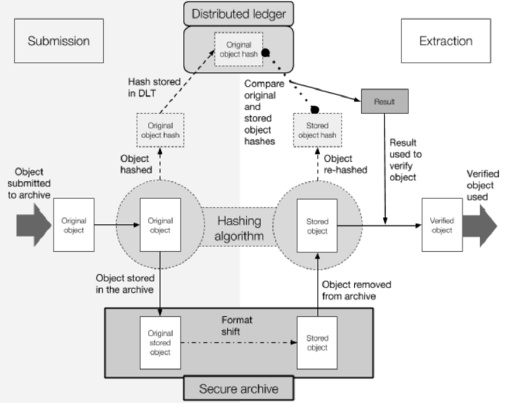
\includegraphics[width=0.5\textwidth]{archangel.png}\label{fig:archangel}
\end{figure}
Within the ARCHANGEL project, a combination of blockchain and artificial intelligence was attempted in a bid to ensure the integrity of audiovisual records. Audiovisual records require a continuous conversion of formats for utilization, and the converted record has a different hash value even with the same content as the original copy if the format is changed. To resolve this problem, the ARCHANGEL project developed the temporal content hash by applying the deep neural network as a kind of artificial intelligence technique \cite[3]{bui2019archangel}.

In this research, the machine learning algorithm was executed with the aim of extracting the content characteristics of audiovisual records irrespective of whether the format was converted. As the unique value is extracted by capturing the content characteristics regardless of the format conversion, TCH was the concept suggested for the first time by the ARCHANGEL project \cite[3]{bui2019archangel}. This research proposed the application of TCH for the replacement of SHA 256 hash values as a means to guarantee the integrity of audiovisual records \cite[4]{wang2021research}.
\section{Provenance framework for the IOT}
\cite{Sigwart2020} proposed a generic data provenance framework for the IoT. Their approach is to store provenance records on the Ethereum blockchain. Their approach is to store provenance records on the blockchain, with the goal of immutable provenance records for supply chains or other use cases \cite[4]{Sigwart2020}. 

The framework is interesting for my thesis, since the framework can be adapted to store fixity information instead of provenance data by simply adapting the smart contract code of the project, which is publicy available on github \footnote{\url{https://github.com/msigwart/iotprovenance}}.
\section{Remote Data Integrity Checking Scheme}
\cite{zhao2020blockchain} proposed a blockchain based remote data integrity checking scheme. Their scheme consists of three phases, including setup, storage and verification phase, this scheme may be of great importance for my work because it integrates well with the work of Sigwart et al. 2020 in terms of design goals. The detail of each phase in their scheme is described as follows: (1) Setup phase, where the public parameter of the elliptic curve group is uploaded to the blockchain. (2) Storage phase, where the data owner signs the data blocks and uploads them to a cloud storage. (3) Verification phase, where the data owner downloads the data or desires to check the integrity of the individual data. The auditing process is done by verifying the signature of the data blocks by the data owner.